\chapter{}

\section{membuat workspace}
\begin{enumerate}
    \item Membuat  sebuah data di Microsoft excel
    \item Membuka oracle apex online. Klik get started for free dan klik request a free workspace
    \item Masukkan data kamu seperti nama depan, nama belakang, email aktif dan nama workspacenya harus beda dengan yang sudah ada
    \item Di no 1 klik yes, di no 2 klik no
    \item Masukkan tujuan mu membuat workspace ini
    \item Klik kotak accept
    \item Klik submit
\item Setelah klik submit cek email dan untuk membuat aplikasi bisa masuk melalui pesan yang dikirimoracle ke email. Atau dengan membuka akun workspace kalian.
    \begin{figure}[!htbp]
        \centering
        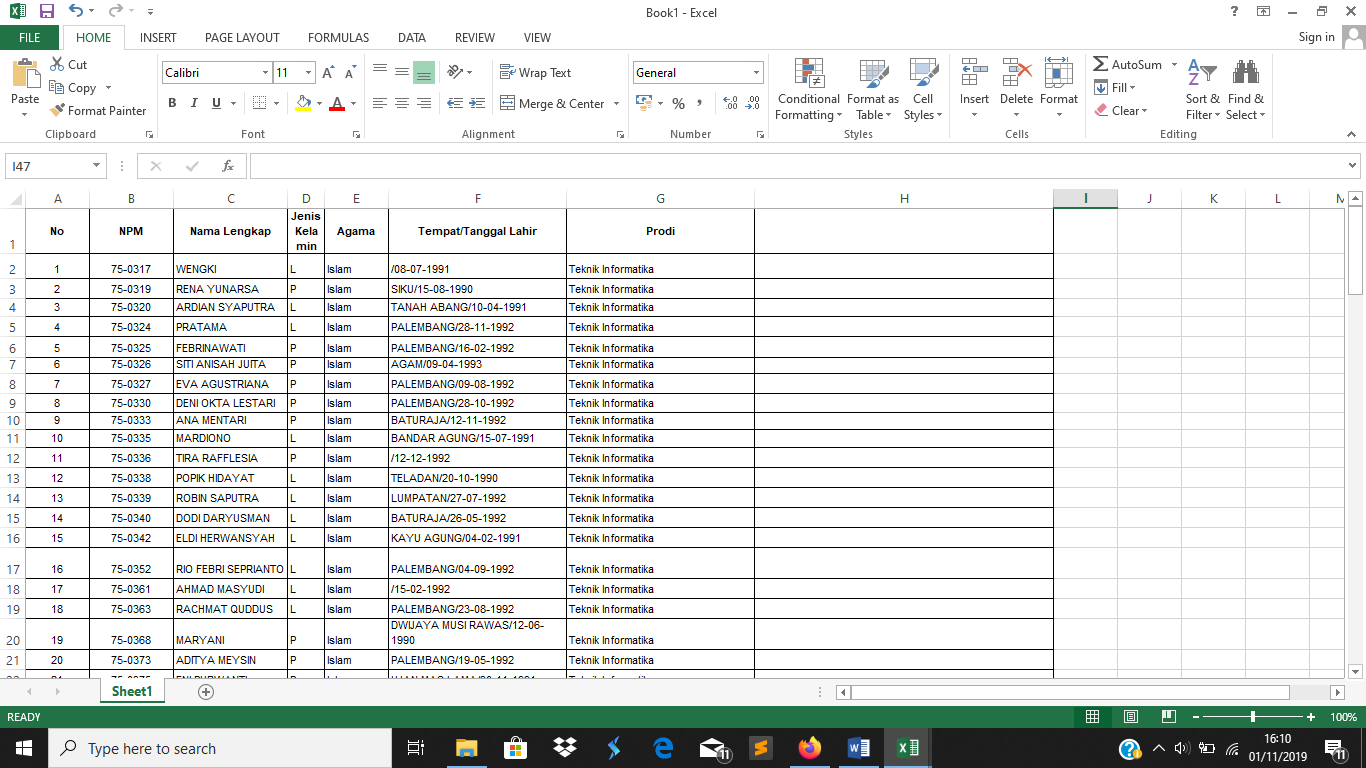
\includegraphics[scale=0.3]{figure/1.png}
        \caption{Caption}
        \label{fig:my_label}
    \end{figure}
   
    \begin{figure}[!htbp]
        \centering
        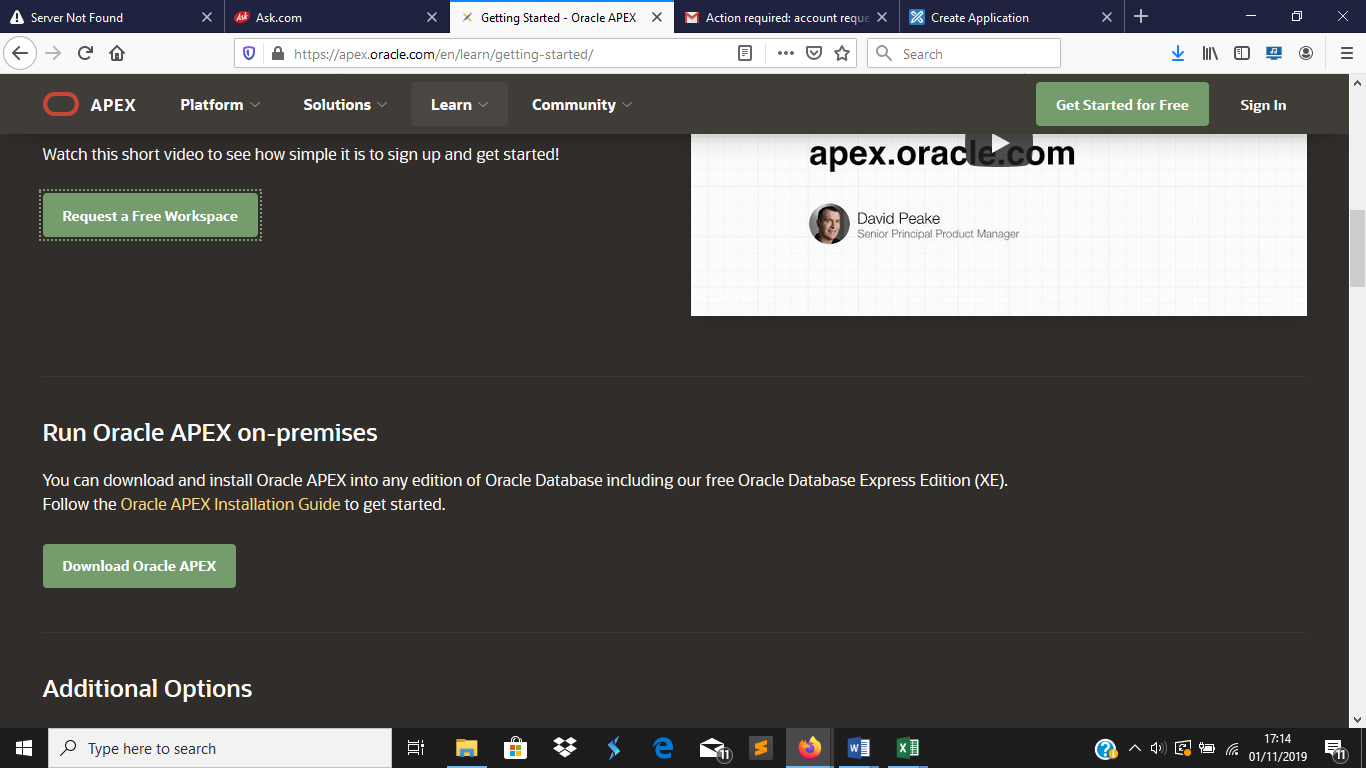
\includegraphics[scale=0.3]{figure/2.png}
        \caption{Caption}
        \label{fig:my_label}
    \end{figure}
    
    \begin{figure}[!htbp]
        \centering
        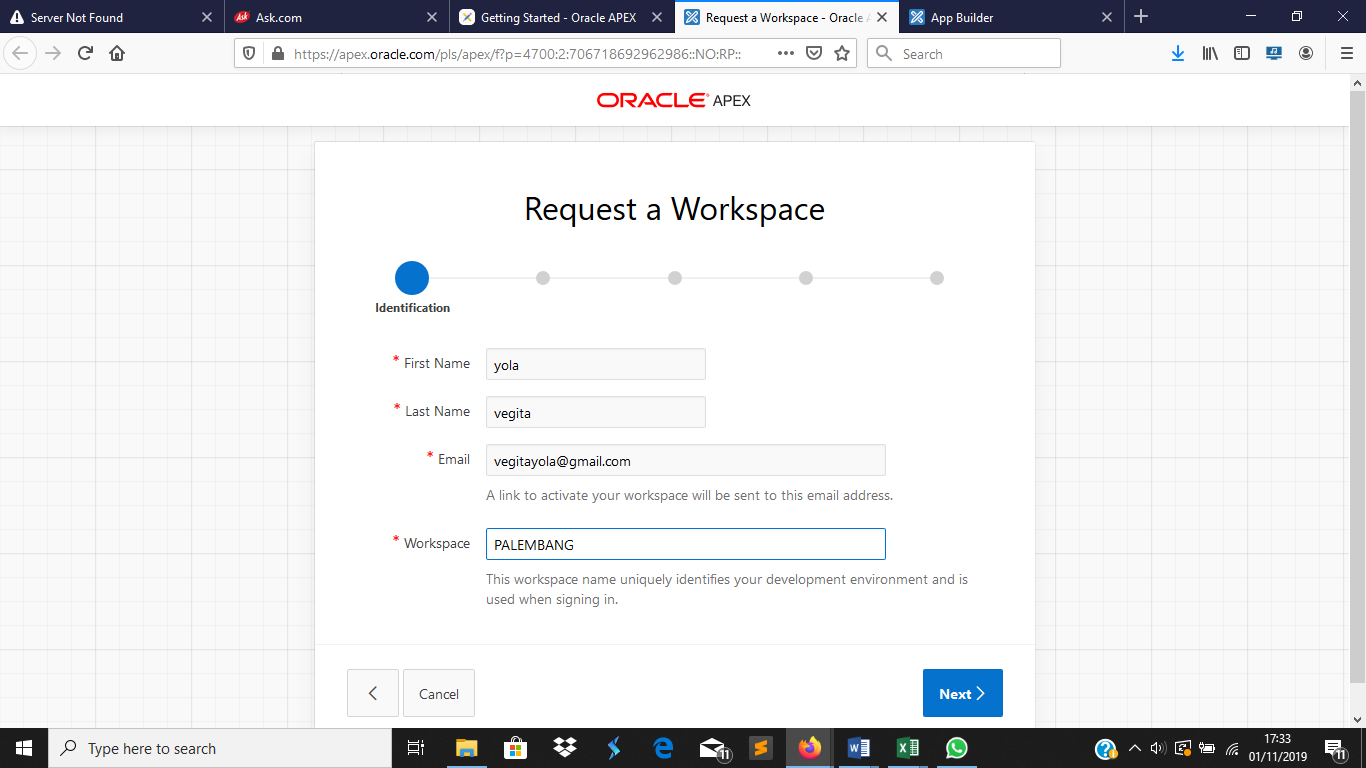
\includegraphics[scale=0.3]{figure/3.png}
        \caption{Caption}
        \label{fig:my_label}
    \end{figure}
    
    \beh\begin{figure}[!htbp]
        \centering
        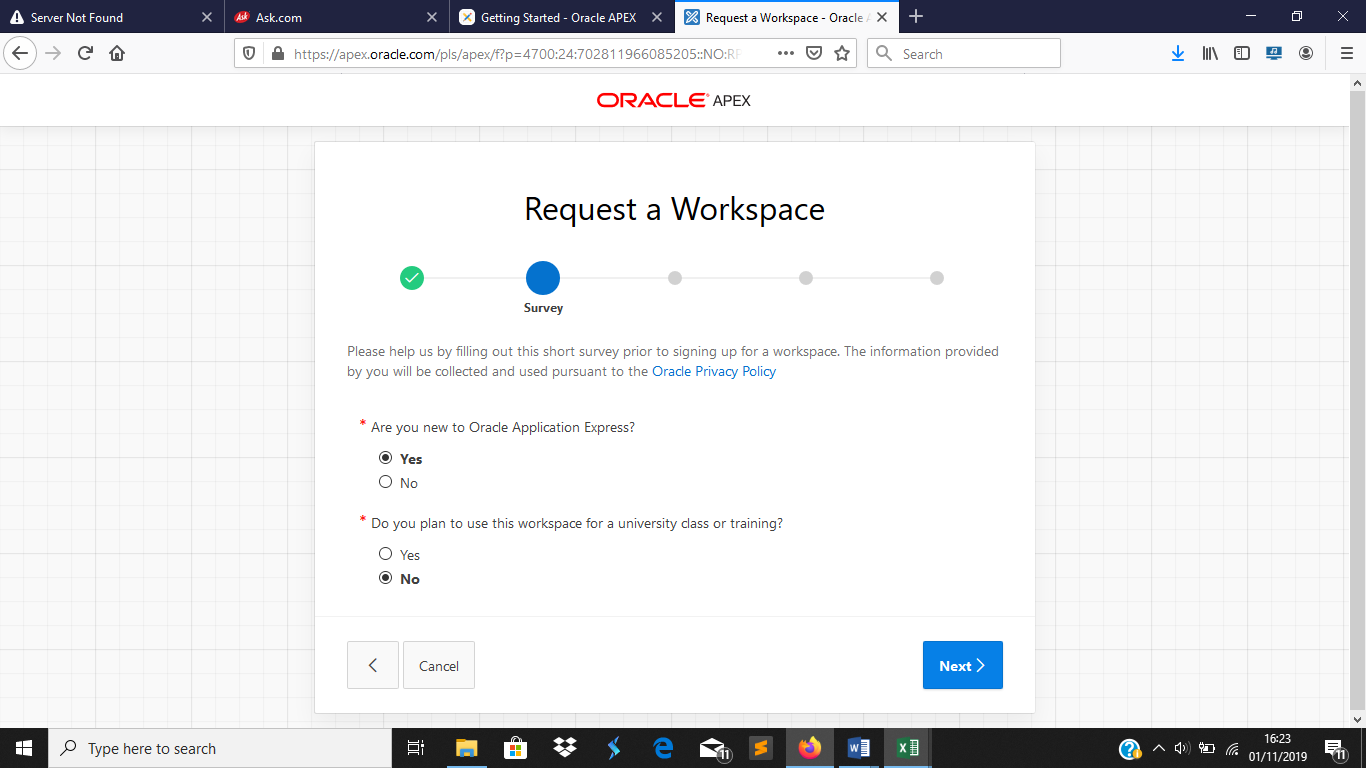
\includegraphics[scale=0.3]{figure/4.png}
        \caption{Caption}
        \label{fig:my_label}
    \end{figure}
    
    \begin{figure}[!htbp]
        \centering
        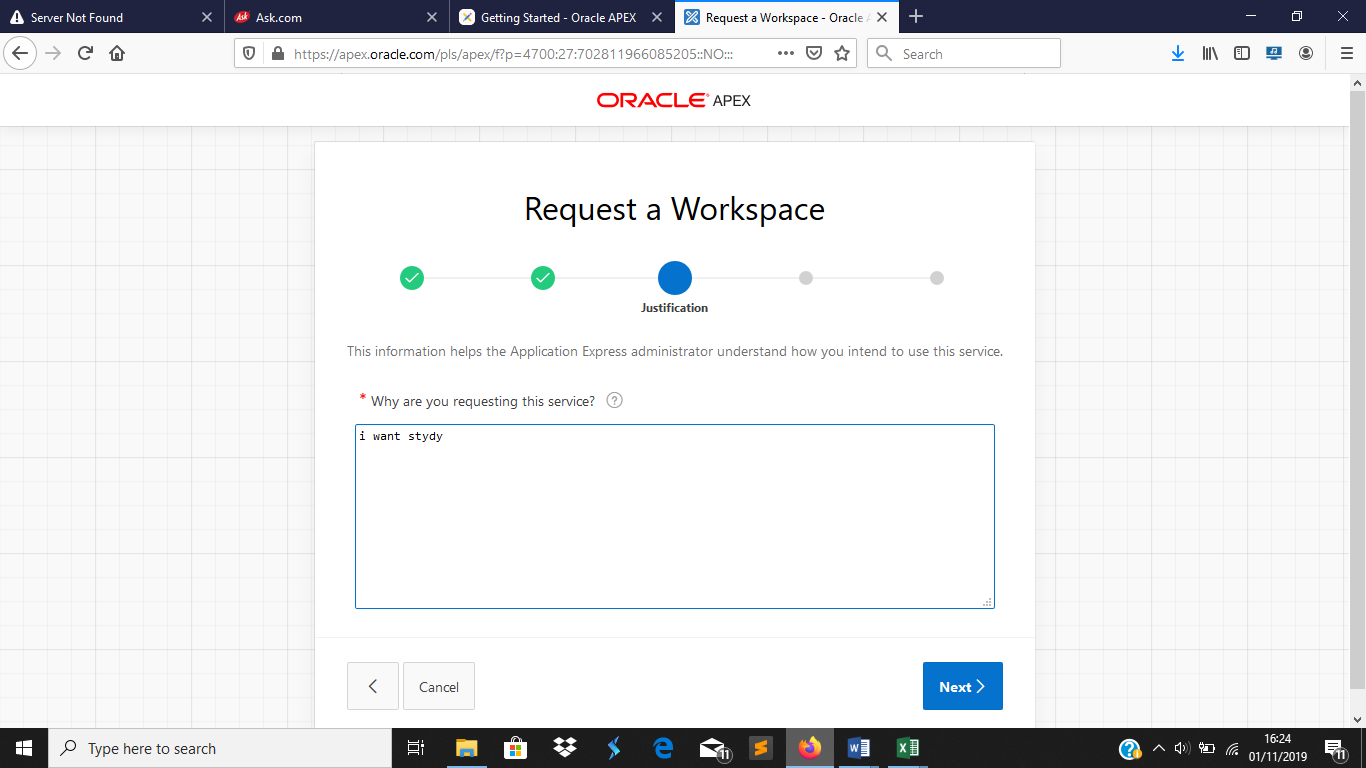
\includegraphics[scale=0.3]{figure/5.png}
        \caption{Caption}
        \label{fig:my_label}
    \end{figure}
    
    \begin{figure}[!htbp]
        \centering
        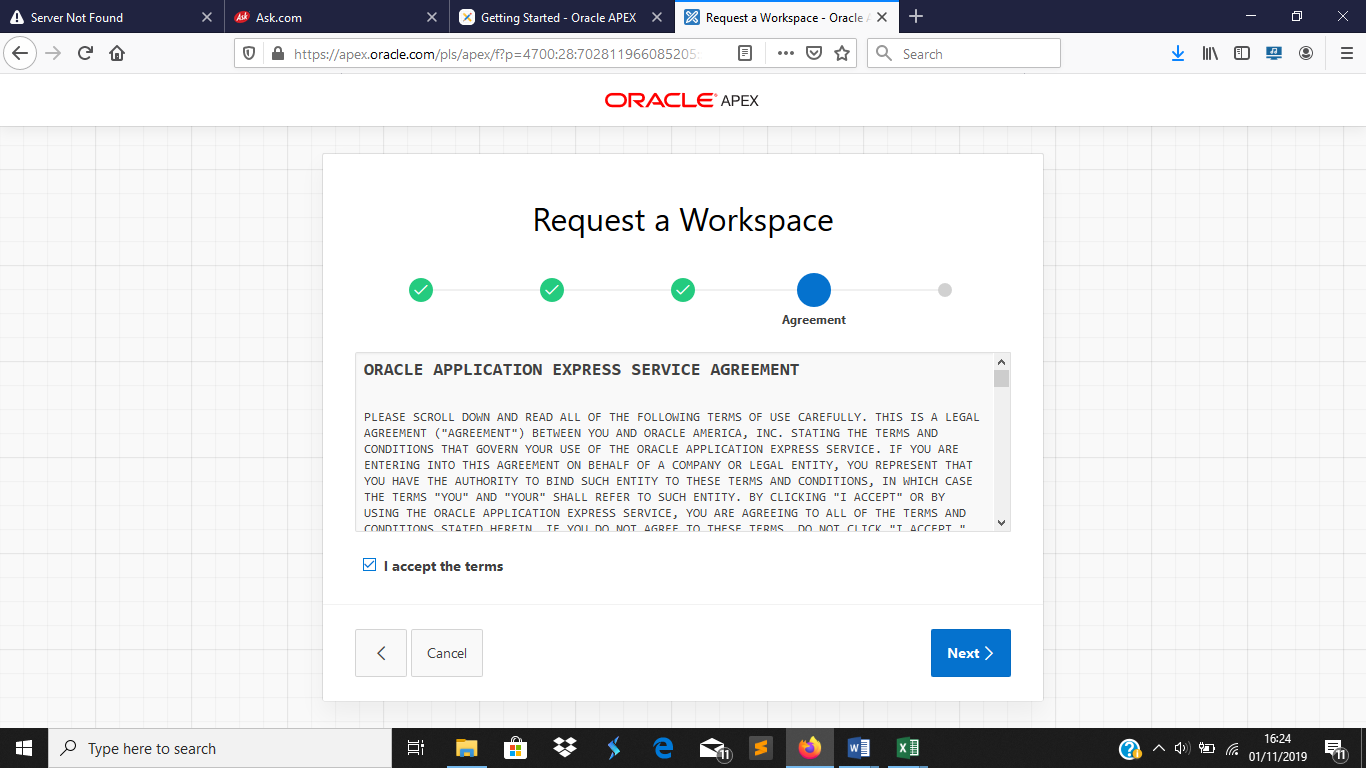
\includegraphics[scale=0.3]{figure/6.png}
        \caption{Caption}
        \label{fig:my_label}
    \end{figure}
    
    \begin{figure}[!htbp]
        \centering
        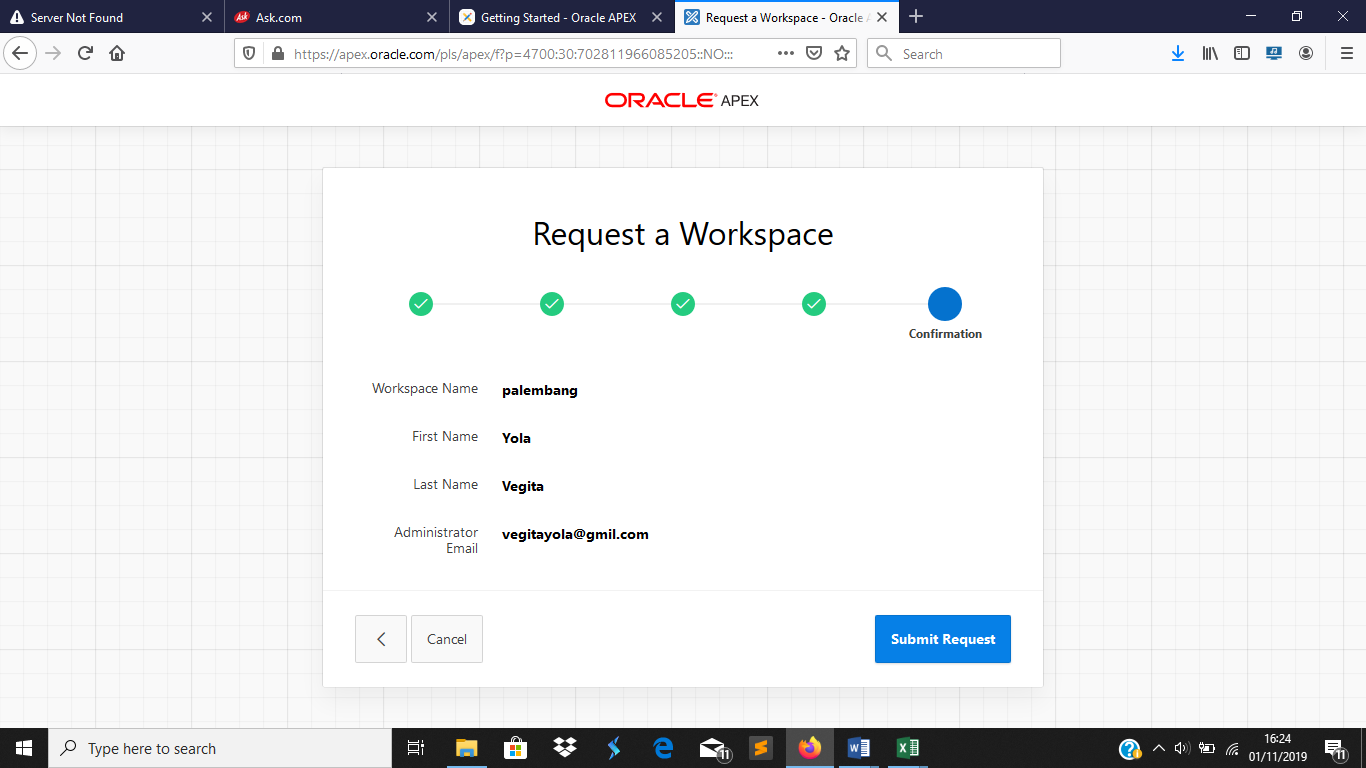
\includegraphics[scale=0.3]{figure/7.png}
        \caption{Caption}
        \label{fig:my_label}
    \end{figure}
    \begin{figure}[!htbp]
        \centering
        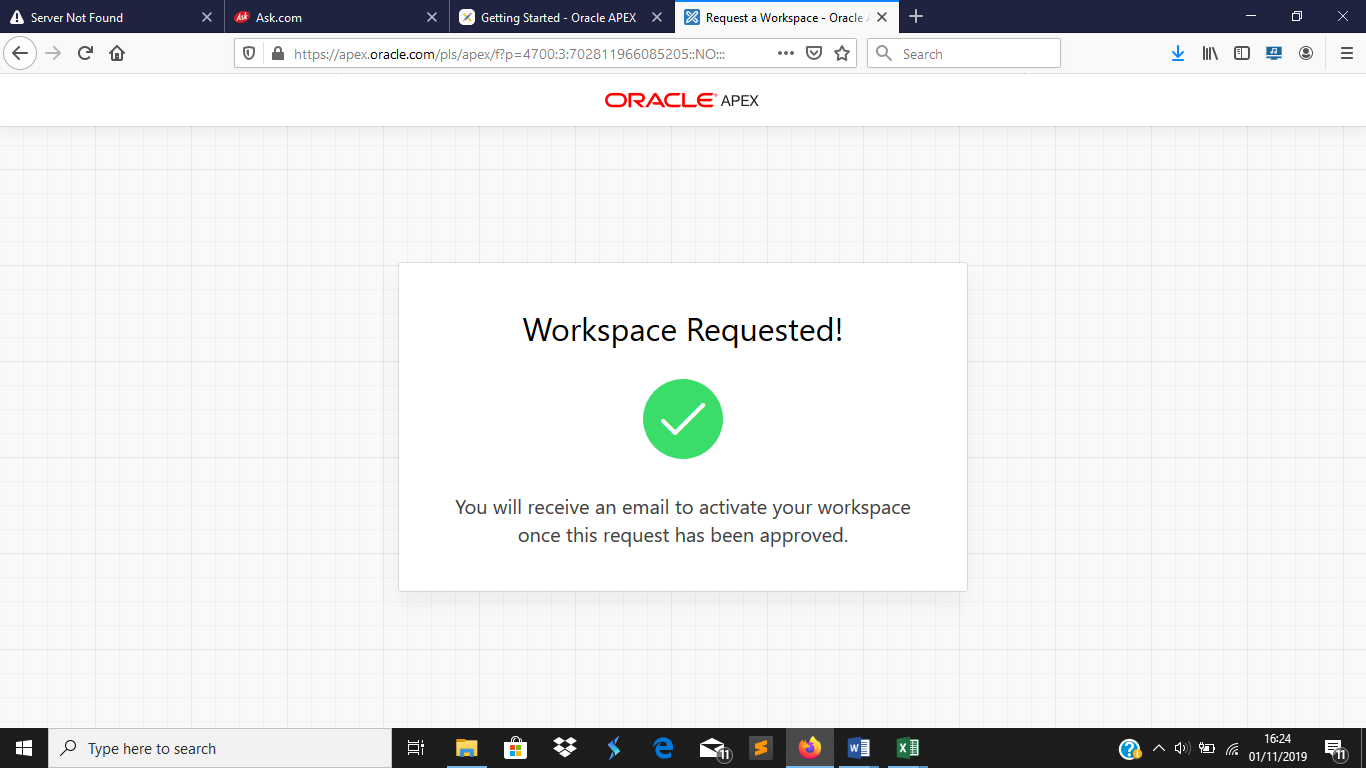
\includegraphics[scale=0.3]{figure/8.png}
        \caption{Caption}
        \label{fig:my_label}
    \end{figure}
    
    \begin{figure}[!htbp]
        \centering
        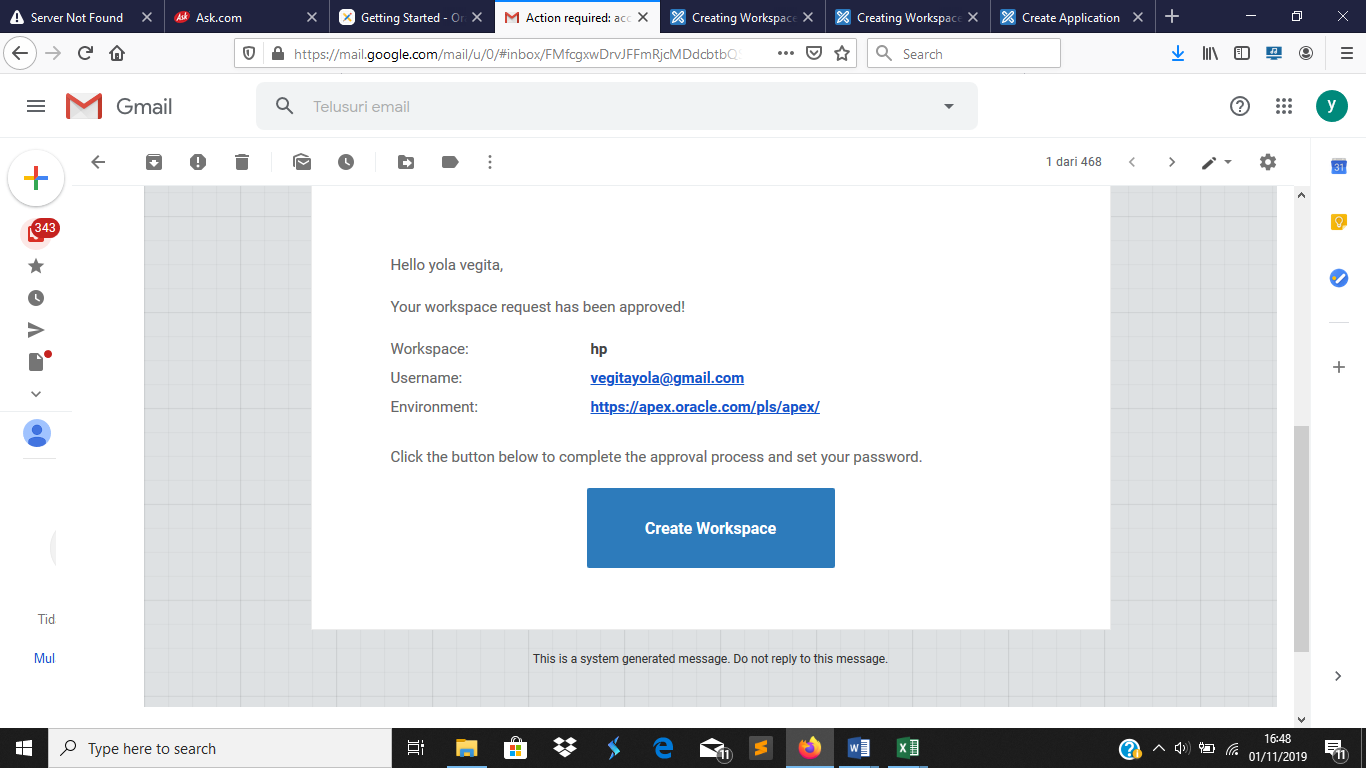
\includegraphics[scale=0.3]{figure/9.png}
        \caption{Caption}
        \label{fig:my_label}
    \end{figure}{}
\end{enumerate}


\section{Membuat Aplikasi Dengan Menggunakan Oracle Apex}
 Link akses : https://apex.oracle.com/pls/apex/f?p=78955:1:700273504181116::::: \par
\par User : vegitayola@gmail.com \par Pwd : #Yola123
\begin{enumerate}
\item Klik app bulder

\item Klik create
\item Klik from a file
\item Klik Choose file, lalu pilih data yang sudah kamu buat sebelumnya

\item Beri nama table nya
\item Proses pembuatan aplikasi berhasil. Klik create
\item Klik create application
\item Klik run application
\item Login dengan menggunakan user dan pwd
\item Pembuatan app selesai.
\begin{figure}[!htbp]
    \centering
    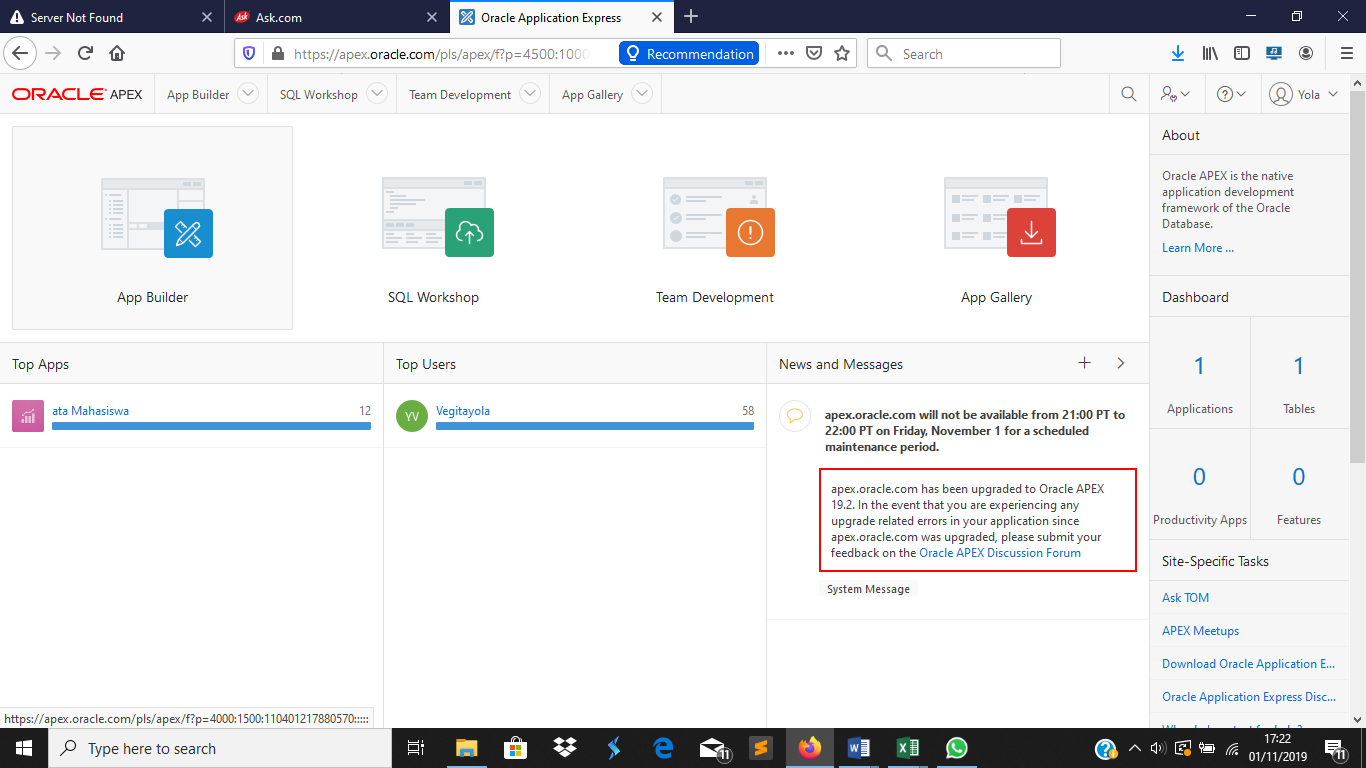
\includegraphics[scale=0.3]{figure/10.png}
    \caption{Caption}
    \label{fig:my_label}
\end{figure}

\begin{figure}[!htbp]
    \centering
    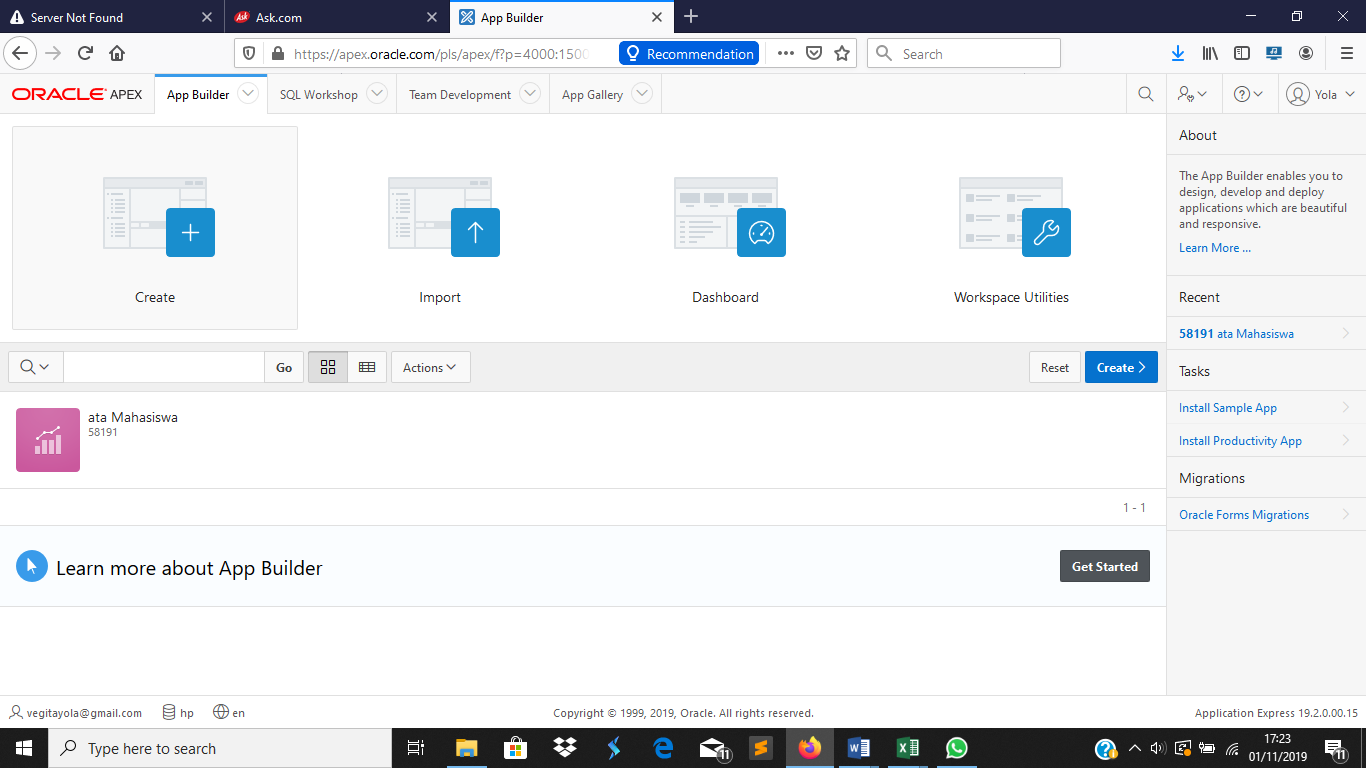
\includegraphics[scale=0.3]{figure/11.png}
    \caption{Caption}
    \label{fig:my_label}
\end{figure}

\begin{figure}[!htbp]
    \centering
    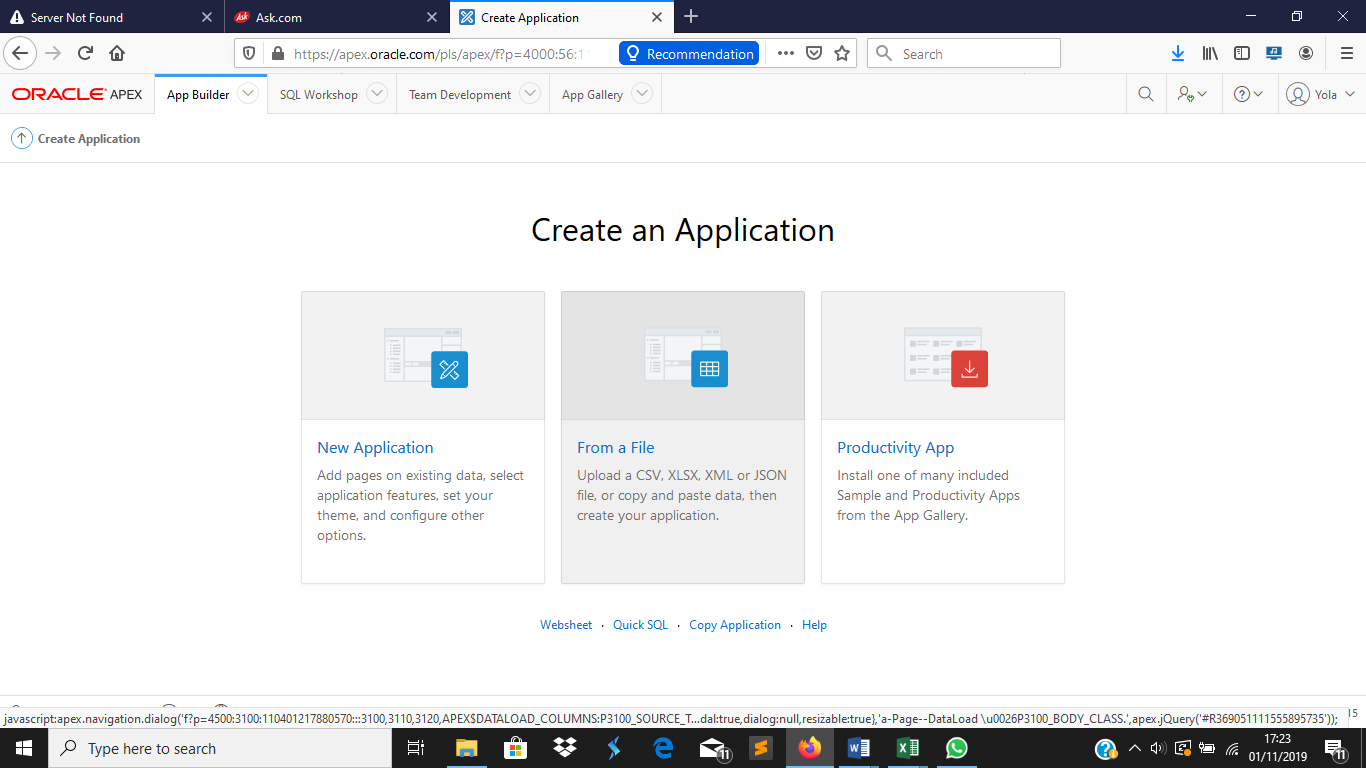
\includegraphics[scale=0.3]{figure/12.png}
    \caption{Caption}
    \label{fig:my_label}
\end{figure}

\begin{figure}[!htbp]
    \centering
    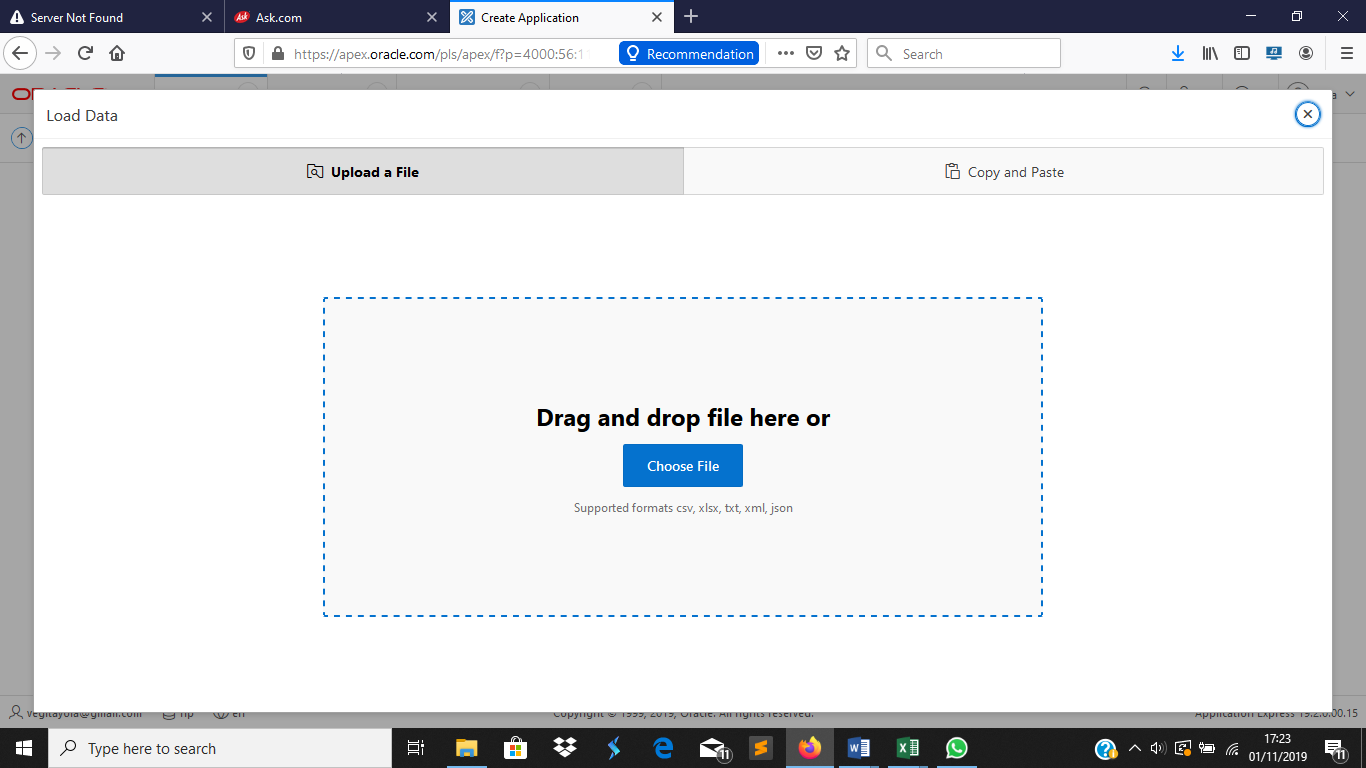
\includegraphics[scale=0.3]{figure/13.png}
    \caption{Caption}
    \label{fig:my_label}
\end{figure}
\begin{figure}[!htbp]
    \centering
    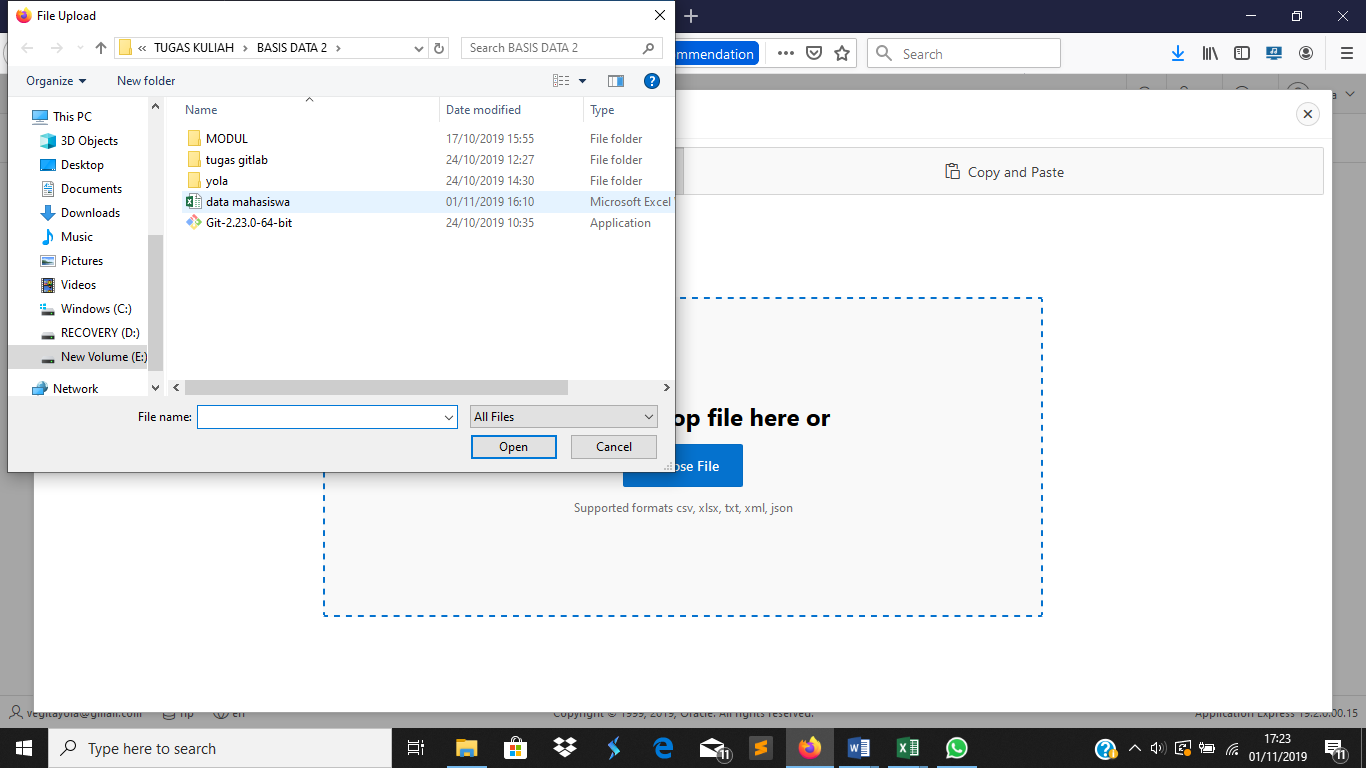
\includegraphics[scale=0.3]{figure/14.png}
    \caption{Caption}
    \label{fig:my_label}
\end{figure}

\begin{figure}[!htbp]
    \centering
    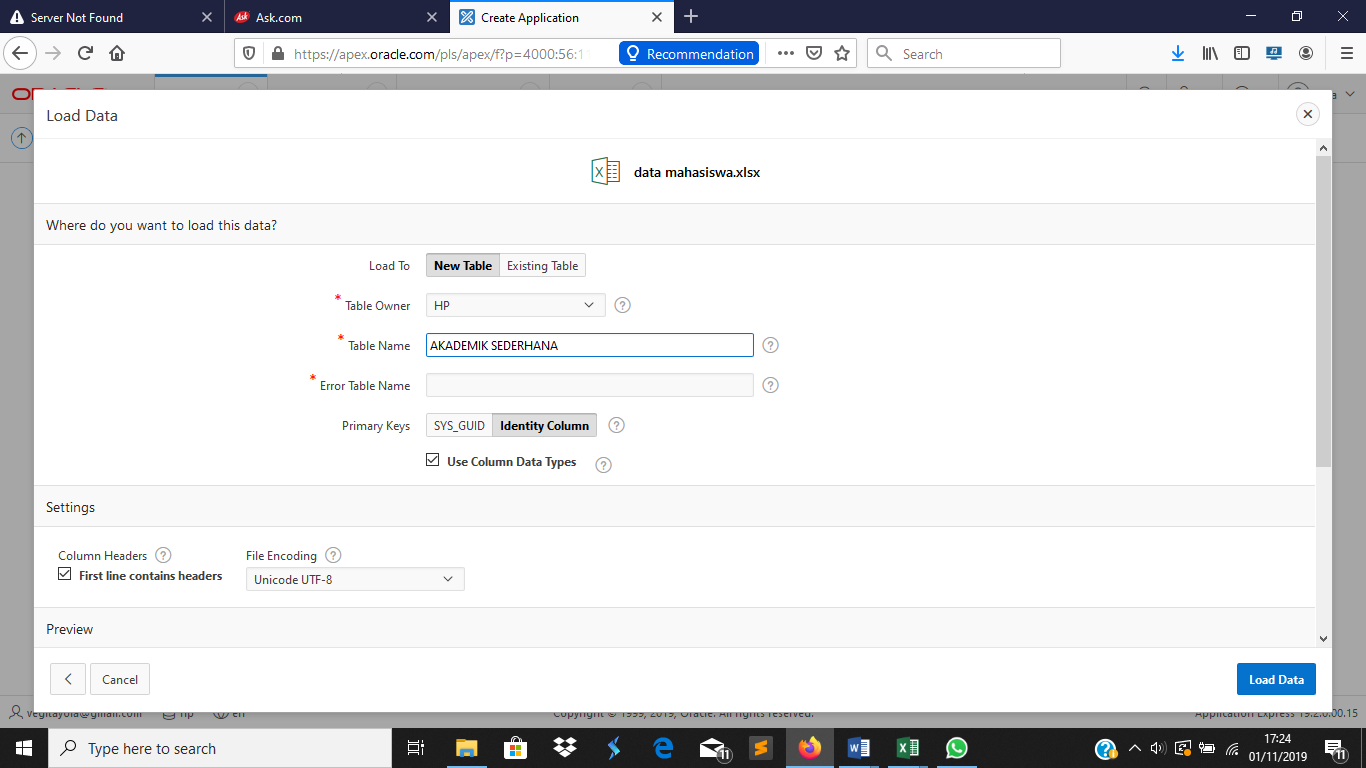
\includegraphics[scale=0.3]{figure/15.png}
    \caption{Caption}
    \label{fig:my_label}
\end{figure}

\begin{figure}[!htbp]
    \centering
    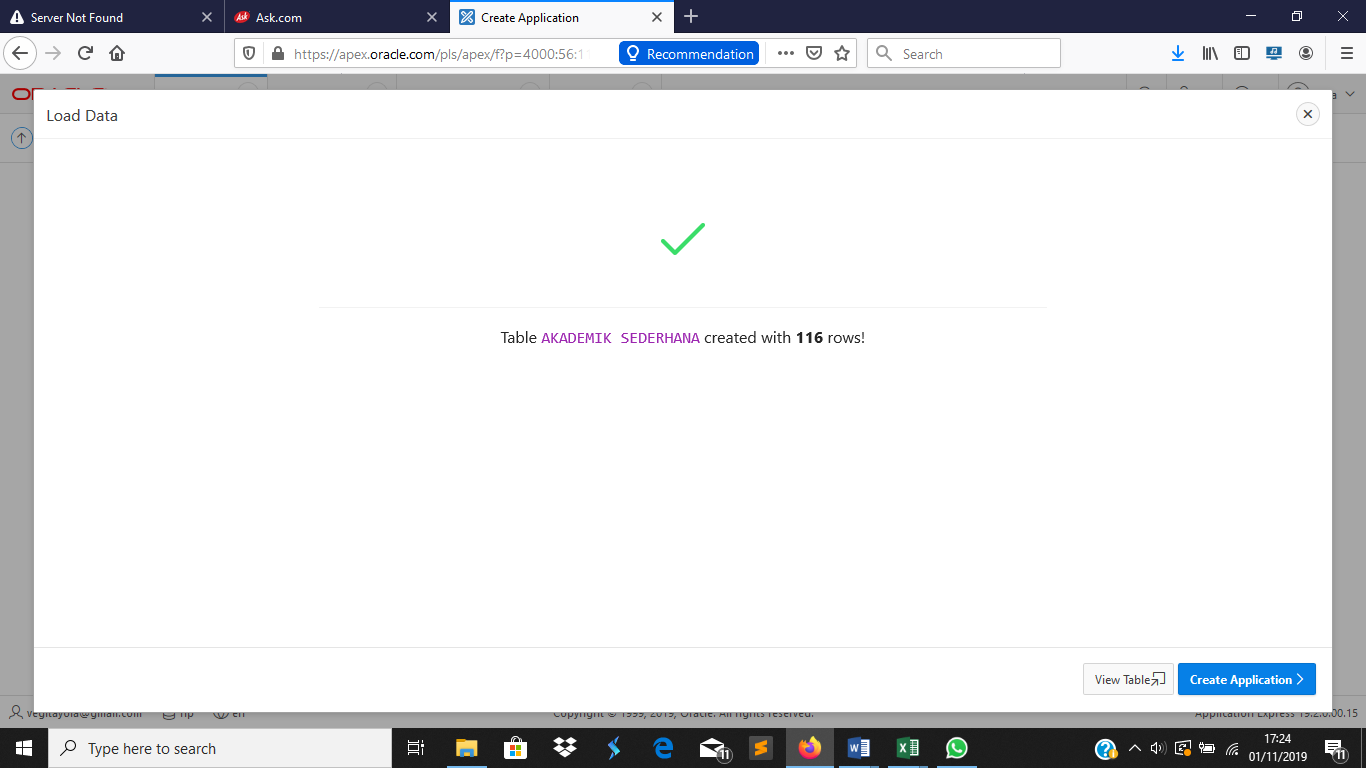
\includegraphics[scale=0.3]{figure/16.png}
    \caption{Caption}
    \label{fig:my_label}
\end{figure}[]

\begin{figure}[!htbp]
    \centering
    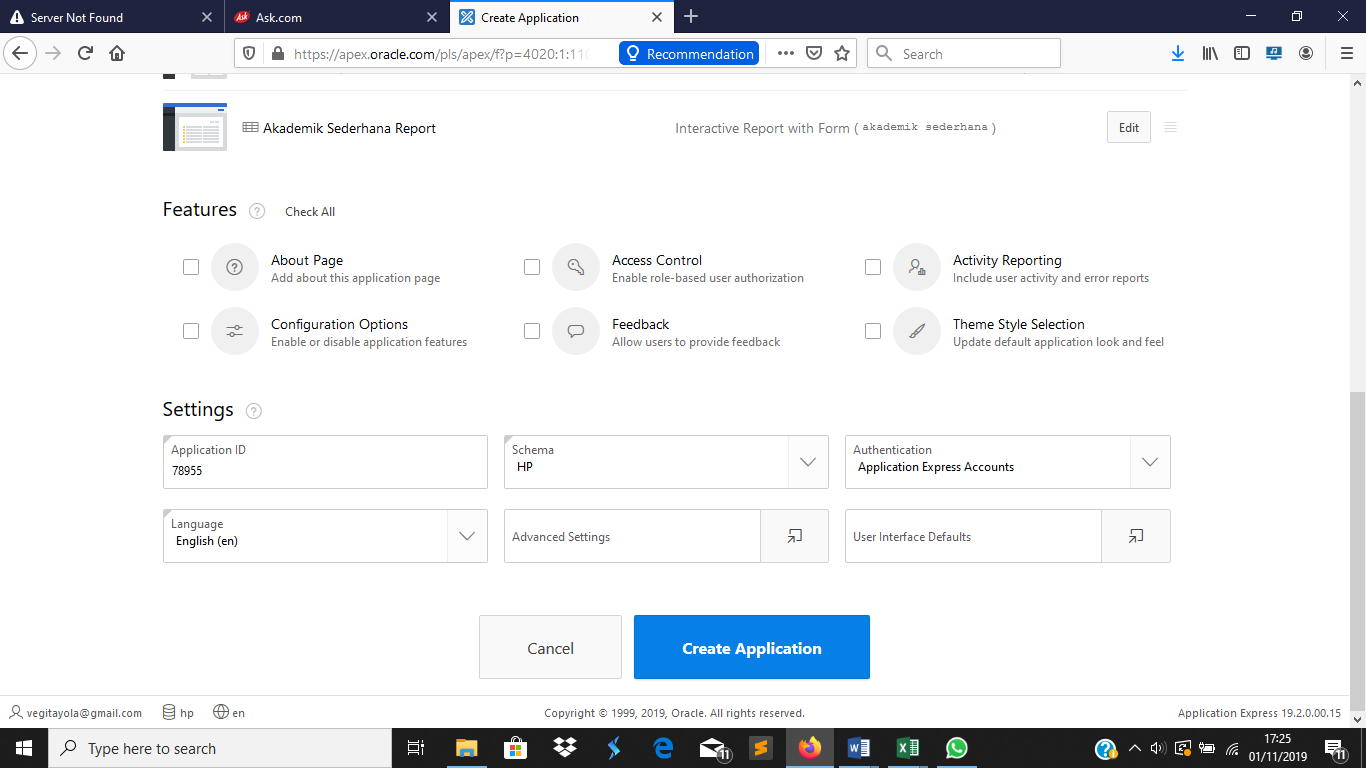
\includegraphics[scale=0.3]{figure/17.png}
    \caption{Caption}
    \label{fig:my_label}
\end{figure}

\begin{figure}[!htbp]
    \centering
    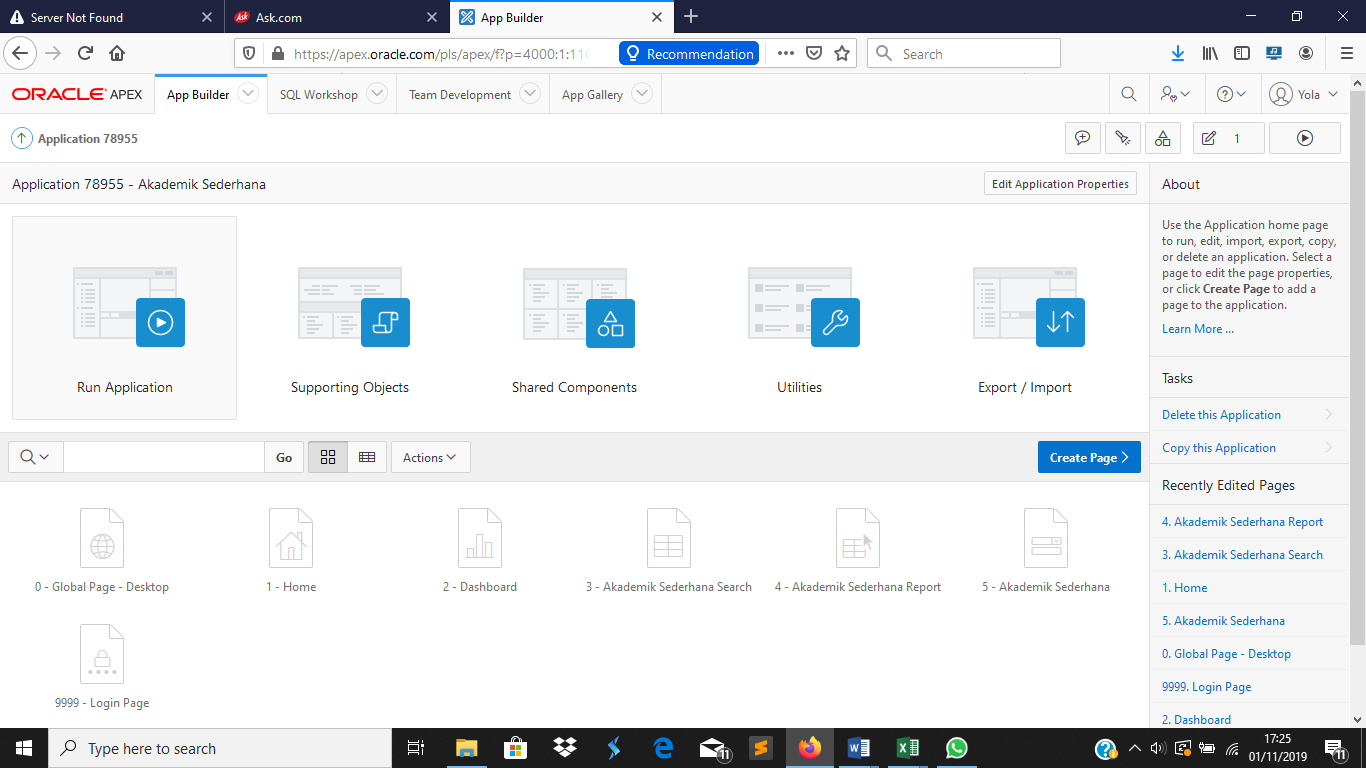
\includegraphics[scale=0.3]{figure/18.png}
    \caption{Caption}
    \label{fig:my_label}
\end{figure}

\begin{figure}[!htbp]
    \centering
    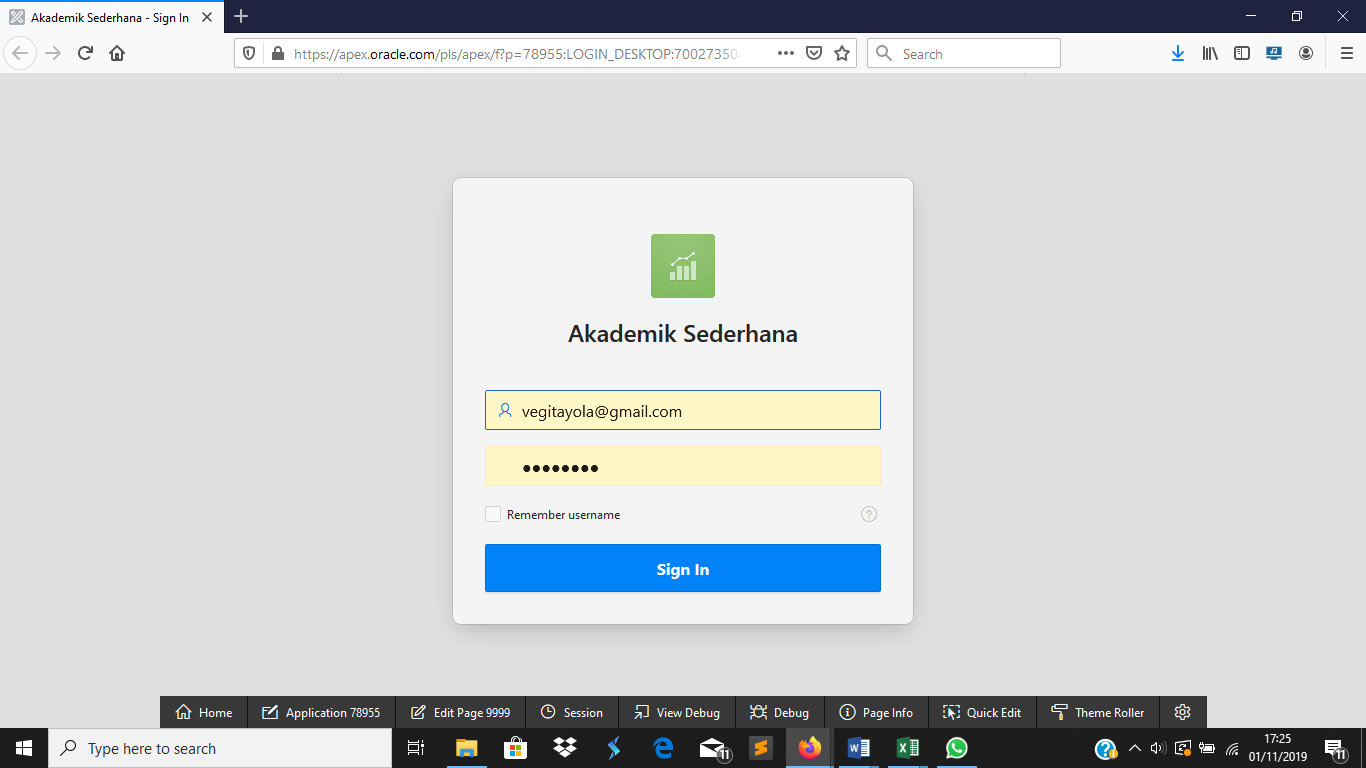
\includegraphics[scale=0.3]{figure/19.png}
    \caption{Caption}
    \label{fig:my_label}
\end{figure}

\begin{figure}[!htbp]
    \centering
    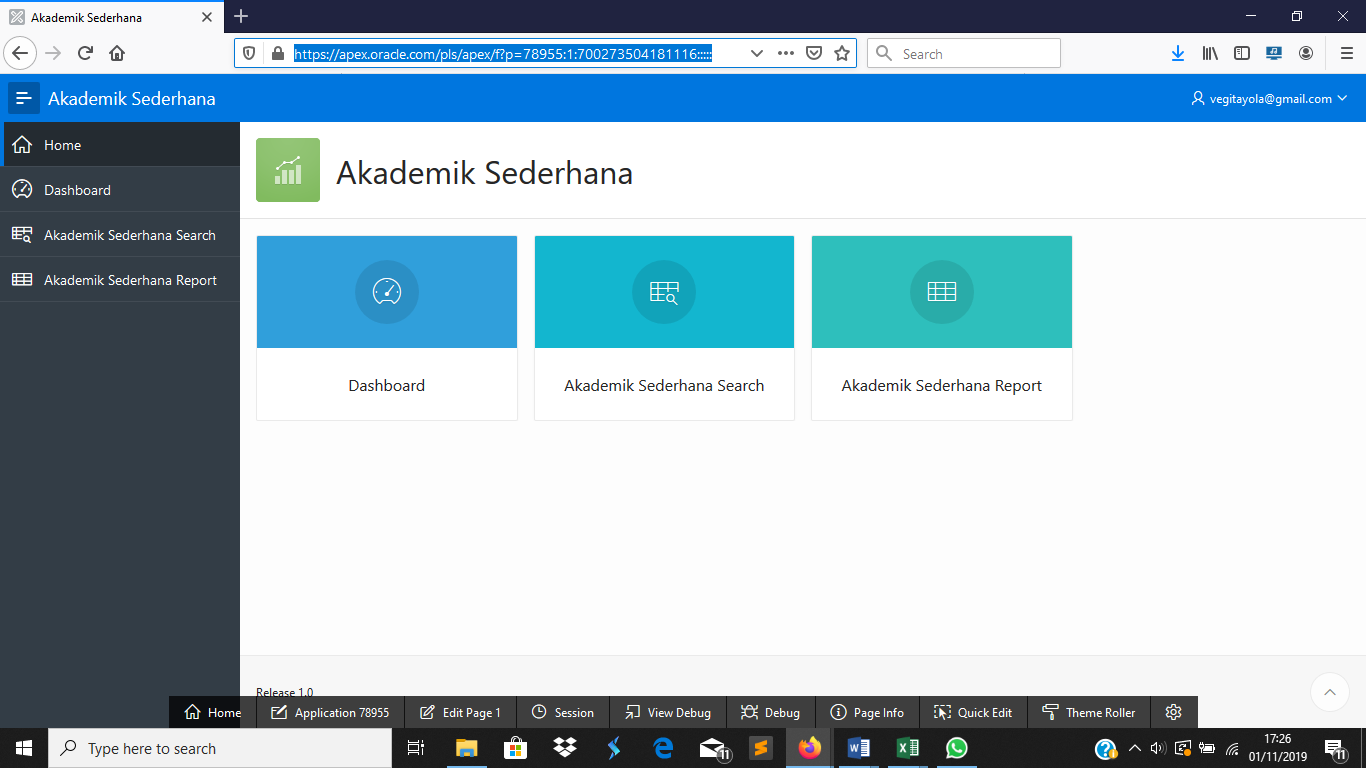
\includegraphics[scale=0.3]{figure/20.png}
    \caption{Caption}
    \label{fig:my_label}
\end{figure}
\begin{figure}[!htbp]
    \centering
    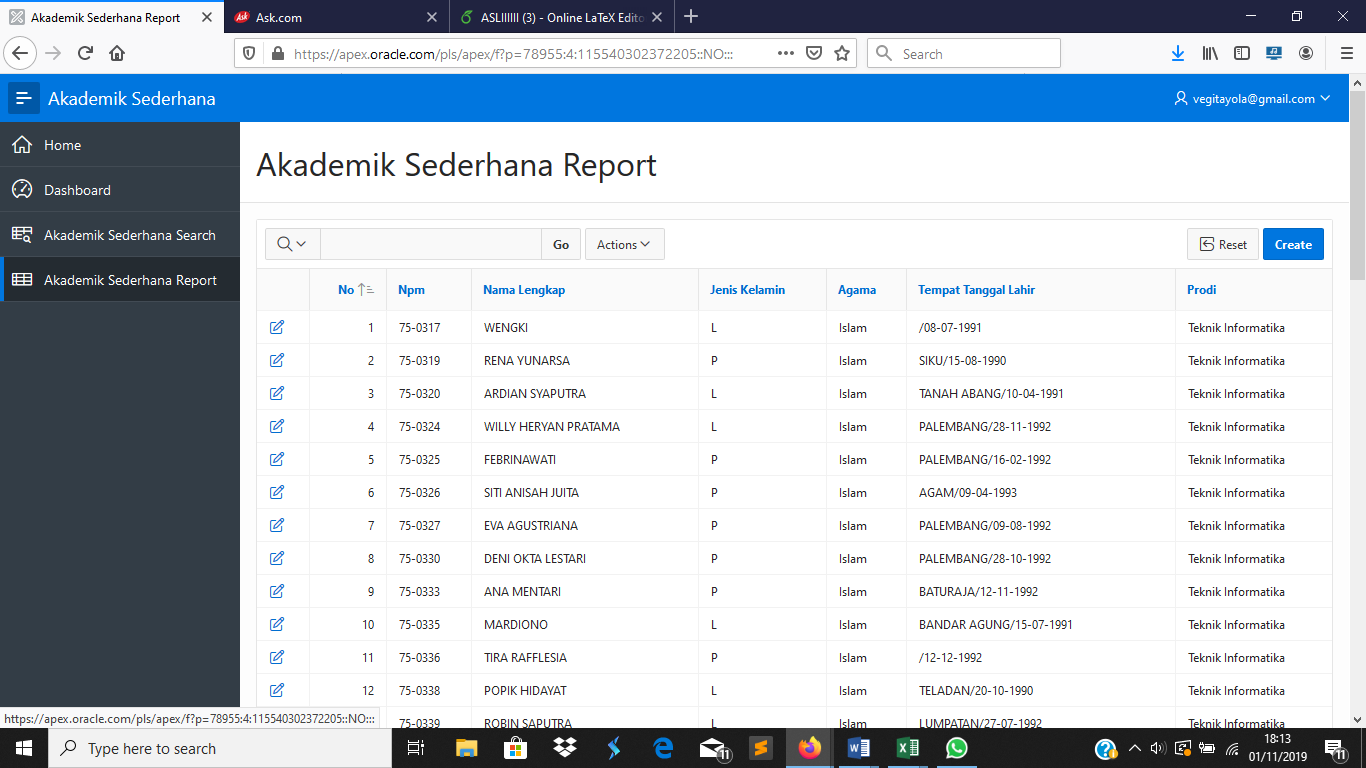
\includegraphics[scale=0.3]{figure/21.png}
    \caption{Caption}
    \label{fig:my_label}
\end{figure}
\end{enumerate}


